\documentclass[11pt,a4paper,twoside]{article}
\usepackage[T1]{fontenc}
\usepackage{isabelle,isabellesym}
\usepackage{amssymb}

%% Seitenformat:
\setlength{\oddsidemargin}{0cm}         % li. Randabstand auf re. Seiten
\setlength{\textwidth}{16cm}            % Breite des Textes
\setlength{\evensidemargin}{0cm}        % li. Randabstand auf li. Seiten
\setlength{\topmargin}{-0.75cm}         % Abst. Oberkante Blatt - Oberk. Header
\setlength{\headheight}{30pt}           % H\hookrightarrow e des Headers
\setlength{\headsep}{0pt}               % Abst. Header - Text
\setlength{\topskip}{1cm}               % Oberkante Text - Grundlinie 1. Z.
\setlength{\textheight}{23.5cm}         % H\hookrightarrow e des Textes
%%\setlength{\footheight}{0cm}          % H\hookrightarrow e des Footers
\setlength{\footskip}{0cm}              % Abst. Unterk. Text - Unterk. Footer

\usepackage{graphicx}
\usepackage{xspace}

\usepackage{fancyvrb}
\usepackage{fancyhdr}
\usepackage{prooftree}

%%%%%%%%%%%%%%%%%%%%%%%%%%%%%%%%%%%%%%%%%%%%%%%%%%%%%%%%%%%%%%%%%%%%%%%%%%%%%%
% Einstellungen f"ur den Seitenstil (fancyhdr)
%%%%%%%%%%%%%%%%%%%%%%%%%%%%%%%%%%%%%%%%%%%%%%%%%%%%%%%%%%%%%%%%%%%%%%%%%%%%%%
\pagestyle{fancyplain}

%% Setzen von Dicke und Breite der Linie unter der Kopfzeile.
\renewcommand{\headrulewidth}{1.6pt}
\newfont{\kopffont}{cmr10}  % zum Justieren des Fonts
\renewcommand{\sectionmark}[1]{\markboth{\kopffont\thesection\ #1}{}}
\renewcommand{\subsectionmark}[1]{\markright{\kopffont\thesubsection\ #1}}

%% Setzen der Kopflayouts ("`~\\"' erzeugt zus"atzlichen vertikalen Abstand).
\lhead[\kopffont\thepage]%  erscheint links auf
                                            %  geraden Seiten
      {\fancyplain{}{\rightmark}}  % erscheint links auf
                                            % ungeraden Seiten 

\chead{} % erscheint zentriert auf beiden Seiten

\rhead[\fancyplain{}{\leftmark}]% erscheint rechts auf
                                          % geraden Seiten
      {\kopffont\thepage}% erscheint rechts auf
                                           % ungeraden Seiten 
\cfoot{}  % im Fu"s soll nichts stehen
%%%%%%%%%%%%%%%%%%%%%%%%%%%%%%%%%%%%%%%%%%%%%%%%%%%%%%%%%%%%%%%%%%%%%%%%%%%%%%

% this should be the last package used
\usepackage{pdfsetup}
% urls in roman style, theory text in math-similar italics
\urlstyle{rm}
\isabellestyle{it}

\usepackage{my_logic}

\renewcommand{\jive}{\textsc{Jive}\xspace}
\newcommand{\isabelleP}{\textsc{Isabelle}\xspace}
\newcommand{\isabelleH}{\textsc{Isabelle/HOL}\xspace}
\newcommand{\javake}{\textsc{Java-KE}\xspace}

\begin{document}

% to be added for the TechReport
\title{%{\normalsize Interner Bericht xxx/05}\\
%{\normalsize Technische Universit\"at Kaiserslautern}\\[1cm]
Jive Data and Store Model\\[1cm]
~}
\author{
Norbert Schirmer\\TU M\"unchen\\schirmer@informatik.tu-muenchen.de
\and
Nicole Rauch\\TU Kaiserslautern\\rauch@informatik.uni-kl.de}

\date{}

\maketitle

\begin{abstract}
% This Internal Report
This document presents  the formalization of an object-oriented data and store model in \isabelleH.
This model is being used in the \textbf{J}ava \textbf{I}nteractive \textbf{V}erification \textbf{E}nvironment, \jive.
\end{abstract}

\thispagestyle{empty}


\cleardoublepage

\markboth{\kopffont Contents}{\kopffont Contents}
\tableofcontents
\markboth{\kopffont Contents}{\kopffont Contents}

\parindent 0pt\parskip 0.5ex

\cleardoublepage

\section{Introduction}

\jive \cite{Meyer.Poetzsch-Heffter00architecture,Jive} is a verification system that is being developed at the 
University of Kai\-sers\-lautern and at the ETH 
Z\"urich. It is an interactive special-purpose theorem 
prover for the verification of object-oriented programs on the basis of a partial-correctness Hoare-style programming logic.
\jive operates on \javake \cite{Poetzsch-Heffter.Gaillourdet.EA05hoare},
a desugared subset of sequential Java which contains all important features of object-oriented languages
(subtyping, exceptions, static and dynamic method invocation, etc.). \jive is written in Java and currently has a size of about 40,000 lines of code.

\jive is able to operate on completely unannotated programs, allowing the user to dynamically add specifications. It is also possible to preliminarily annotate programs with invariants, pre- and postconditions using the specification language JML 
\cite{Leavens.BakerEA99jml}. In practice, a mixture of both techniques is employed, in which the user extends and refines the pre-annotated specifications during the verification process.
The program to be verified, together with the specifications, is translated to Hoare sequents. Program and pre-annotated specifications are translated during startup, while the dynamically added specifications are translated whenever they are entered by the user.
Hoare sequents have the shape
$\Sequent{A}{\bP}{\mathtt{pp}}{\bQ}$ and express that for all states $S$ that fulfill $\bP$, if the execution of the program part $\mathtt{pp}$ terminates,
the state that is reached when $pp$ has been evaluated in $S$ must
fulfill $\bQ$. The so-called assumptions $\cl{A}$ are used to prove recursive methods.

\jive's logic contains so-called Hoare rules and axioms. The rules consist of one or more Hoare sequents that represent the assumptions of the rule, and a Hoare sequent which is the conclusion of the rule. Axioms consist of only one Hoare sequent; they do not have assumptions. Therefore, axioms represent the known facts of the Hoare logic.

To prove a program specification, the user directly works on the program source code.
Proofs can be performed in backward direction and in forward direction. In backward direction, an initial open proof goal is reduced to new, smaller open subgoals by applying a rule. This process is repeated for the smaller subgoals until eventually each open subgoal can be closed by the application of an axiom. If all open subgoals are proven by axioms, the initial goal is proven as well.

In forward direction, the axioms can be used to establish known facts about the statements of a given program.
The rules are then used to produce new facts from these already known facts. This way, facts can be constructed for parts of the program.

A large number of the rules and axioms of the Hoare logic is related to the structure of the program part that is currently being examined. Besides these, the logic also contains rules that manipulate the pre- or postcondition of the examined subgoal without affecting the current program part selection.
A prominent member of this kind of rules is the rule of consequence\footnote{In \jive, the rule of consequence is part of a larger rule which serves several purposes at once. Since we want to focus on the rule of consequence, we left out the parts that are irrelevant in this context.}:
\[
\begin{prooftree}
\bPP \Rightarrow \bP \qquad
\Sequent{A}{\bP}{\mathtt{pp}}{\bQ} \qquad
\bQ \Rightarrow \bQQ
\justifies
\Sequent{A}{\bPP}{\mathtt{pp}}{\bQQ}
\end{prooftree}
\]
It plays a special role in the Hoare logic because it additionally requires implications between stronger and weaker conditions to be proven. 
If a \jive proof contains an application of the rule of consequence, the implication is attached to the proof tree node that documents this rule application; these attachments are called lemmas. 
\jive sends these lemmas to an associated general purpose theorem prover where the user is required to prove them. Currently, \jive supports \isabelleH as associated prover. 
It is required that all lemmas that are attached to any node of a proof tree are proven before the initial goal of the proof tree is accepted as being proven.

In order to prove these logical predicates, \isabelleH
needs a data and store model of \javake. This model acts as an interface
between \jive and \isabelleH. 

The first paper-and-pencil 
formalization
of the data and store model was given in Arnd Poetzsch-Heffter's habilitation thesis 
\cite[Sect. 3.1.2]{Poetzsch-Heffter97specification}. The first machine-supported formalization was performed in
PVS by Peter M\"uller, by translating the axioms given in \cite{Poetzsch-Heffter97specification} 
to axioms in PVS. The formalization
presented in this report extends the PVS formalization.
The axioms have been replaced by conservative extensions and proven lemmas, thus 
there is no longer any possibility to accidentally introduce unsoundness.

Some changes were made to the PVS theories during the conversion. Some were caused due to
the differences in the tools \isabelleH and PVS, but some are more
conceptional. Here is a list of the major changes.

\begin{itemize}
\item In PVS, function arguments were sometimes restricted to subtypes. In \isabelleH,
  unintended usage of functions is left unspecified.

\item In PVS, the program-independent theories were parameterized by the datatypes that were
  generated for the program to be verified. In \isabelleH, we just build on the generated theories. This makes
  the whole setting easier. The drawback is that we have to run the theories
  for each program we want to verify. But the proof scripts are designed in a
  way that they will work if the basic program-dependent theories are generated in the proper
  way. Since we can create an image of a proof session before starting actual
  verification we do not run into time problems either.

\item The subtype relation is based on the direct subtype 
 relation between classes and interfaces. We prove that subtyping forms a partial order. In
  the PVS version subtyping was expressed by axioms that described the subtype relation
  for the types appearing in the Java program to be verified.
\end{itemize}

Besides these changes we also added new concepts to the model. We can
now deal with static fields and arrays. This way, the model supports programming languages that are much richer
than \javake to allow for future extensions of \jive.

Please note that although the typographic conventions in Isabelle
suggest that constructors start with a capital letter while types do
not, we kept the capitalization as it was before (which means that
types start with a capital letter while constructors usually do not)
to keep the naming more uniform across the various \jive-related publications.

The theories presented in this report require the use of \isabelleP 2005. The proofs of lemmas are skipped 
in the presentation to keep it compact.
The full proofs can be found in the original \isabelleP theories. 
% theories can download them \cite{}.

\clearpage

\section{Theory Dependencies}

\begin{center}
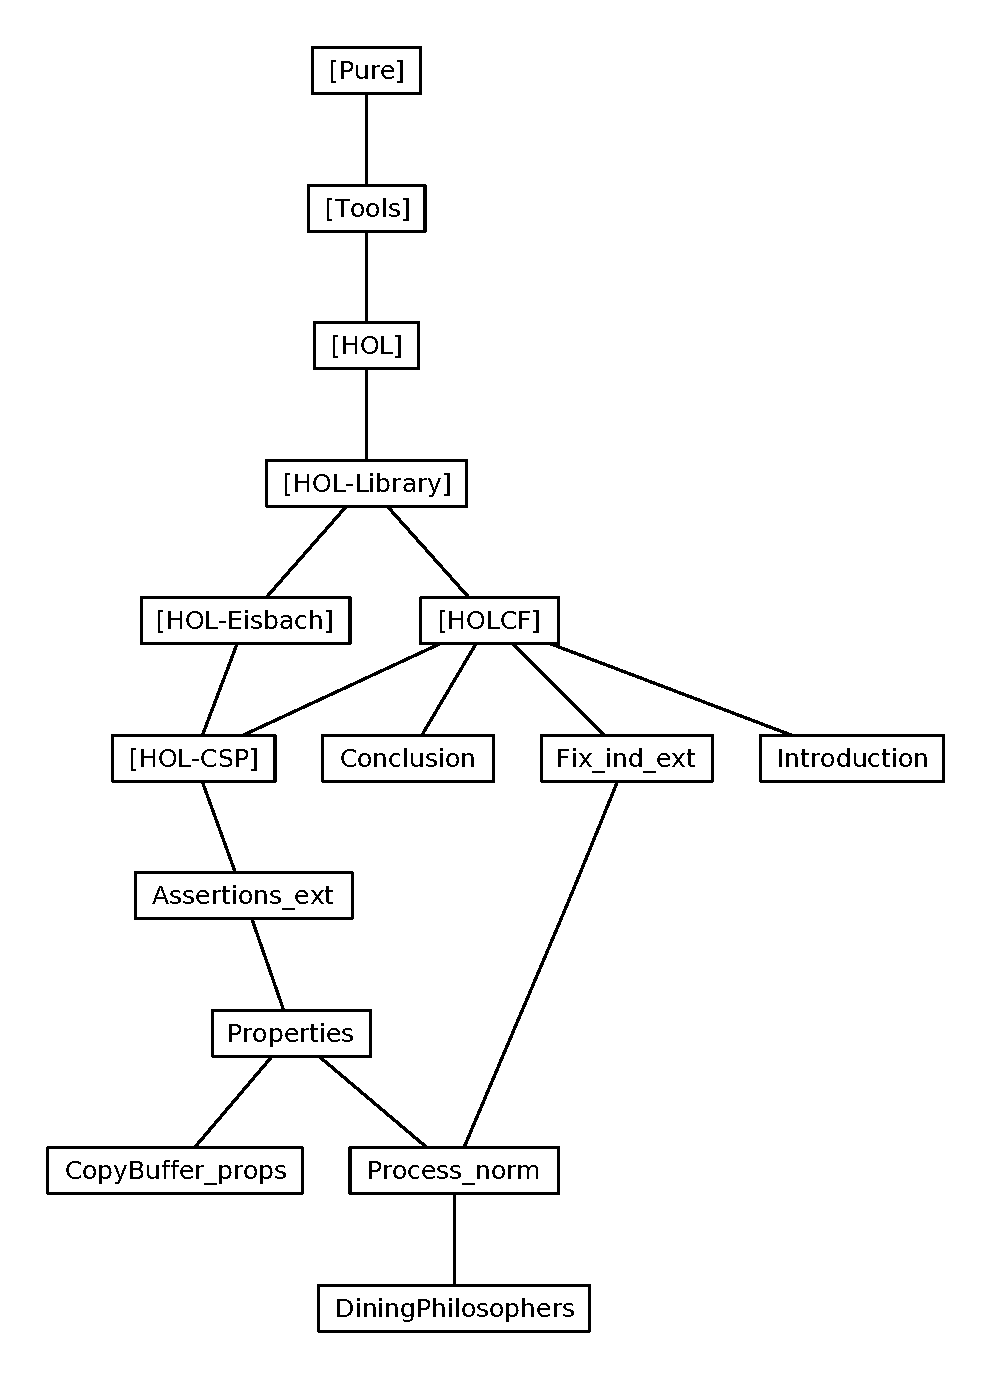
\includegraphics[height=12cm]{session_graph}
%\includegraphics[height=15cm]{session_graph_edited}
\end{center}

The theories ``TypeIds'', ``DirectSubtypes'', ``Attributes'' and ``UnivSpec'' are 
program-dependent and are
generated by the Jive tool. The program-dependent theories  presented in this report are just examples and act as
placeholders. The theories are stored in four different directories:

\begin{tabbing}
XXXXXX\= \kill
Isabelle:\\
\>JavaType.thy \\
\>Subtype.thy \\
\>Value.thy \\
\>JML.thy \\

Isabelle\_Store: \\
\>AttributesIndep.thy \\
\>Location.thy \\
\>Store.thy \\
\>StoreProperties.thy \\

Isa\_$\langle$Prog$\rangle$: \\
\>TypeIds.thy \\
\>DirectSubtypes.thy \\
\>UnivSpec.thy \\

Isa\_$\langle$Prog$\rangle$\_Store: \\
\>Attributes.thy
\end{tabbing}

In this naming convention, the suffix ``\_Store'' denotes those theories that depend on the actual realization of the Store. They have
been separated in order to allow for easy exchanging of the Store realization. The midfix ``$\langle$Prog$\rangle$'' denotes the name
of the program for which the program-dependent theories have been generated. This way, different program-dependent theories can reside
side-by-side without conflicts.

These four directories have to be added to the ML path before loading UnivSpec. This can be done in a
setup theory with the following command (here applied to a program called \texttt{Counter}):

\begin{verbatim}
ML {*
add_path "<PATH_TO_THEORIES>/Isabelle";
add_path "<PATH_TO_THEORIES>/Isabelle_Store";
add_path "<PATH_TO_THEORIES>/Isa_Counter";
add_path "<PATH_TO_THEORIES>/Isa_Counter_Store";
*}
\end{verbatim}

This way, one can select the program-dependent theories for the program that currently is to be proven.

\section{The Example Program} \label{example-program}

The program-dependent theories are generated for the following example program:

\VerbatimInput[fontsize=\small]{Counter.java}

% include generated text of all theories
\input{session}

\bibliographystyle{alpha}
\markboth{\kopffont References}{\kopffont References}
\bibliography{root}

\end{document}
